\documentclass{report}
\usepackage{graphicx}
\usepackage{listings}
\usepackage{xcolor}
\graphicspath{ {./immagini/} }

\title{Homework 1}
\author{Crepaldi Giorgio, Fiandro Andrea, Francois Jeanpierre}
\begin{document}

\maketitle
\tableofcontents

\chapter{Principal Component Visualization}
\subsection{Data standardization}
  The first step is to \textit{standardize} the data, in order to apply correctly the PCA algorithm.
  We found that the function \textit{transform} provided by the \textit{sklearn} library include this preprocessing operation.

\subsection{Image reprojection}

  The next step is to choose one single image and reproject it using only some components.
  This part is implemented with these lines of code:


  \subparagraph{Reproject the image with a specific number of PC}
  \begin{lstlisting}[language=Python]
    pca_x = PCA(n_pca)
    projected = pca_x.fit_transform(input_matrix)
    x_inv = pca_x.inverse_transform(projected)
  \end{lstlisting}

  \subparagraph{Print the new image beside the original one}
  \begin{lstlisting}[language=Python]
    fig = plt.figure()
    fig.add_subplot(1,2,1)
    plt.imshow(np.reshape(input_matrix[nImg,:]/255.0,(227,227,3)))
    fig.add_subplot(1,2,2)
    plt.imshow(np.reshape(x_inv[nImg,:]/255.0,(227,227,3)))
    plt.show()
  \end{lstlisting}

  \pagebreak
  \paragraph{Image reprojection using the whole dataset}
  This is the representation of a random image reprojected using:

  \begin{itemize}
  \item the first 60 PC
  \item the first 6 PCA
  \item the first 2 PCA
  \item the last 6 PCA
  \end{itemize}
  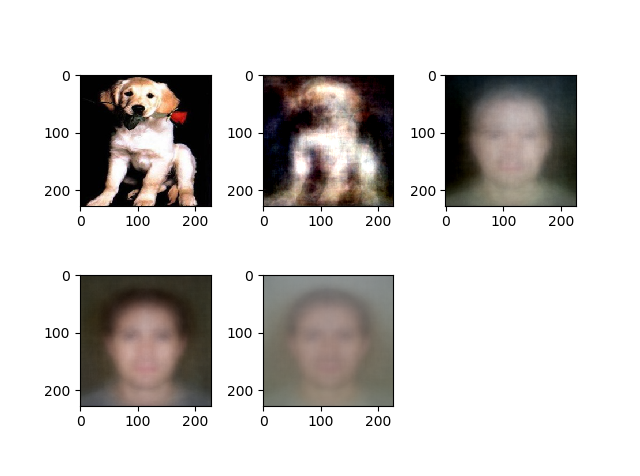
\includegraphics{img_01}
  As we can see, with the first images we have a good representation of the original one. But then we start getting pictures that looks like a human face.
  This behaviour depends on our dataset that is not balanced and includes a lot of faces and few dogs.

  \pagebreak
  \paragraph{Image reprojection using only dogs}
  Here we tried to reproject images using only dog pictures in our dataset.
  This is the result that we get:

  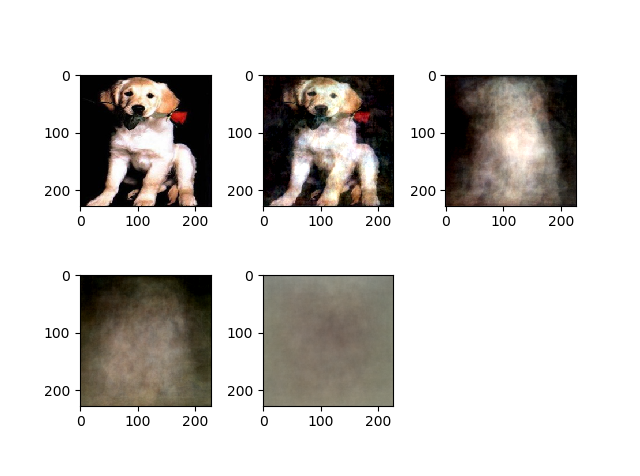
\includegraphics{img_02}

  In this scenario we obviously have a better result.

  \subsection{Scatter plot showing different classes}
  First of all, we define an array that, for each sample, define the class.
  In this case we have 4 classes:
  \begin{itemize}
  \item[\textcolor{red}{\textbullet}] \textcolor{red}{Dogs}
  \item[\textcolor{green}{\textbullet}]\textcolor{green}{Guitar}
  \item[\textcolor{blue}{\textbullet}] \textcolor{blue}{House}
  \item[\textcolor{magenta}{\textbullet}] \textcolor{magenta}{Person}
  \end{itemize}

  \pagebreak

  \paragraph{Scatter plot with first 2 PC}

  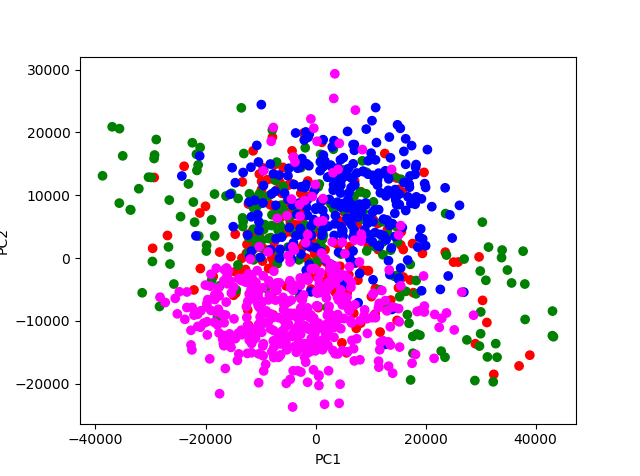
\includegraphics{img_03}

  \paragraph{Scatter plot with third and fourth principal components}

  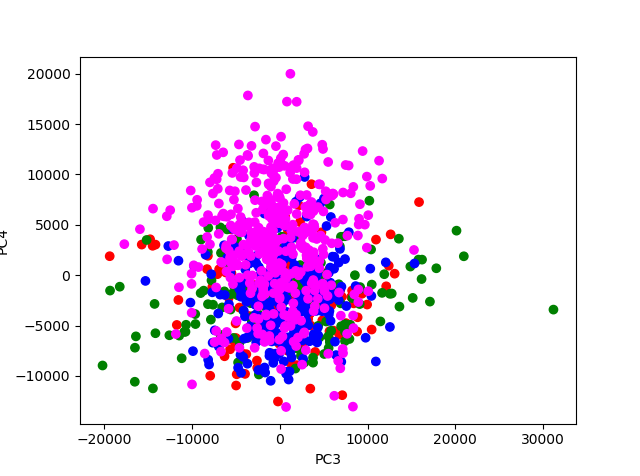
\includegraphics{img_04}

  \paragraph{Scatter plot with tenth and eleventh components}

  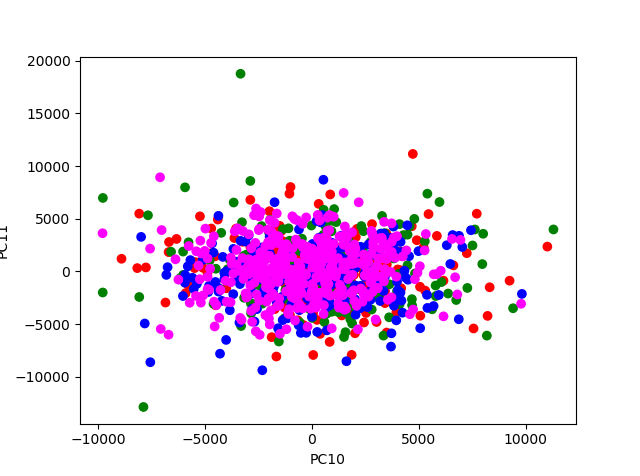
\includegraphics{img_05}


\end{document}
